% \documentclass[11pt,a4paper]{scrartcl}
\documentclass[twoside,10pt,a4paper]{article}
\setlength{\parindent}{0em}
\setlength{\parskip}{1.5em}
\bibliographystyle{apalike}


\renewcommand{\familydefault}{\sfdefault}

\newenvironment{notes}[1][\unskip]{%
\par
\noindent
\textcolor{blue}{\bfseries{Notes - } #1:}
\\ \color{blue}}
{}

\newenvironment{followup}[1][\unskip]{%
\par
\noindent
\textcolor{red}{\bfseries{Follow-up - } #1!!!}
\\ \color{red}}
{}

\newenvironment{question}[1][\unskip]{%
\par
\noindent
\textcolor{orange}{\bfseries{Question - } #1???}
\\ \color{orange}}
{}

\usepackage{mystyle}
% Document Layout
% ---> Document geometry - current setting is set to A4 with relatively narrow margins
\geometry{
  a4paper,
  total={210mm,297mm}, % A4 paper measurement
  left=20mm,
  right=20mm,
  top=25mm,
  bottom=25mm
  }
% ---> Document header and footer setting
\pagestyle{fancy}
\fancyhead[LE,RO]{\leftmark} % Refer to Section/chapter/part on the upperroght of the heading
\fancyhead[RE,LO]{}
\fancyfoot[CE,CO]{}
\fancyfoot[LE,RO]{Page \thepage \, of \pageref{LastPage}} % Print current page and total page number centered in the footer.
% ---> Header and footer horisontal line borders
\renewcommand{\headrulewidth}{1pt}
\renewcommand{\footrulewidth}{0.5pt}

% \definecolor{cell-lghtGry}{RGB}{200,200,200}
%\colorlet{Purple}{blue!40!red}
%\colorlet{Blue}{blue}

\restylefloat{figure}
\restylefloat{table}

% Typesetting code snippets
% The code snippet typesetting below is based on https://www.latextemplates.com/template/code-snippet
% Original Author: This template was created for LaTeXTemplates.com by vel@latextemplates.com
\definecolor{DarkGreen}{rgb}{0.0,0.4,0.0} % Comment color
%\definecolor{highlight}{RGB}{255,251,204} % Code highlight color
\definecolor{highlight}{RGB}{204,255,229} % Code highlight color
\definecolor{Gray}{RGB}{224,224,224}
\definecolor{Purple}{RGB}{255,0,255}
\definecolor{Blue}{RGB}{0,0,255}

\lstdefinestyle{Style1}{ % Define a style for your code snippet, multiple definitions can be made if, for example, you wish to insert multiple code snippets using different programming languages into one document
language=Perl, % Detects keywords, comments, strings, functions, etc for the language specified
backgroundcolor=\color{highlight}, % Set the background color for the snippet - useful for highlighting
basicstyle=\footnotesize\ttfamily, % The default font size and style of the code
breakatwhitespace=false, % If true, only allows line breaks at white space
breaklines=true, % Automatic line breaking (prevents code from protruding outside the box)
captionpos=b, % Sets the caption position: b for bottom; t for top
commentstyle=\usefont{T1}{pcr}{m}{sl}\color{DarkGreen}, % Style of comments within the code - dark green courier font
deletekeywords={}, % If you want to delete any keywords from the current language separate them by commas
%escapeinside={\%}, % This allows you to escape to LaTeX using the character in the bracket
firstnumber=1, % Line numbers begin at line 1
frame=single, % Frame around the code box, value can be: none, leftline, topline, bottomline, lines, single, shadowbox
frameround=tttt, % Rounds the corners of the frame for the top left, top right, bottom left and bottom right positions
keywordstyle=\color{Blue}\bf, % Functions are bold and blue
morekeywords={}, % Add any functions no included by default here separated by commas
numbers=left, % Location of line numbers, can take the values of: none, left, right
numbersep=10pt, % Distance of line numbers from the code box
numberstyle=\tiny\color{Gray}, % Style used for line numbers
rulecolor=\color{black}, % Frame border color
showstringspaces=false, % Don't put marks in string spaces
showtabs=false, % Display tabs in the code as lines
stepnumber=5, % The step distance between line numbers, i.e. how often will lines be numbered
stringstyle=\color{Purple}, % Strings are purple
tabsize=2, % Number of spaces per tab in the code
}

% Create a command to cleanly insert a snippet with the style above anywhere in the document
\newcommand{\insertcode}[2]{\begin{itemize}\item[]\lstinputlisting[caption=#2,label=#1,style=Style1]{#1}\end{itemize}} % The first argument is the script location/filename and the second is a caption for the listing


\pagenumbering{roman}

\begin{document}

  % title ans pharagraps section
  \begin{titlepage}
  \begin{center}


      {\bfseries{\Huge{Deliverable: Analysis of Individual Criteria}}}

    
      {\bfseries{\LARGE{IT Infrastructure Maturity}}}


      {\Large{by}}

    \begin{author}
      \author{\Large{Dale P. Bada}}
    \end{author}


    \vspace*{2.5cm}
    Submitted for Assessment in


    \begin{title}
        \title{\bfseries{\huge{UC1ST1103 - Studio 1}}}
    \end{title}

    \vspace*{2.5cm}
    at


    \Large{Noroff University Collegge}

    \vfill


    \begin{figure}[h!]
      \centering
      
\includegraphics[height=50pt]{Noroff-Logo.png}
    \end{figure}


  \end{center}
\end{titlepage}

  

  % \frontmatter
  % front page, title, table of content etc. will have separate page numbering.
  \tableofcontents
  
  \newpage

  % \listoffigures % uncomment to create list of figures
  % \listoftables % uncomment to create list of tables

  % main document will be rendered with the files listed in this section
  % \mainmatter

  \newpage
  \pagenumbering{arabic}
  \setcounter{page}{1}
  \section{Introduction}

{\huge{Course: UC1PR2101 Programming and Databases}}

S02-PR2-2020

\subsection{Key dates}

\begin{tabular}{r @{} c}
    Duration: & 6 weeks\\
    Start: & 2021-01-04\\
    End: & 2021-02-15\\
    Formative assessment: & TBD\\
    Assessment 1 - Submission date: & TBD\\
    Assessment 2 - Submission date: & TBD\\
\end{tabular}

\subsection{Course Tutors}

\begin{tabular}{r @{} l}
    Course leader: & Johan Van Niekerk\\
    Course lecturer: & Rayne Reid\\
    Course tutor: & Konstantin Lenchik\\
    course tutor: & Mariya Chirchenkova\\
    Support tutor: & Sohail Naseem (KRS)\\
    Support tutor: & Arash Mithraian (OSL)\\
\end{tabular}

\subsubsection{Study goals}

\begin{itemize}
    \item Working with database (SQLite)
        \begin{itemize}
            \item Acquire fundamental skill about working with databases
            \item How to design as simple normalized database
            \item Understand database storage and data structure
            \item Understand database Normalization
            \item Be able to query and interface with databases
            \item How to script and automate database connection, mangagement and datamining
            \item Automate data manipulation and analysis, generating reports and statitics etc on data in databases, dataframes etc.
            \item Understanding and being able to manage and  work with databases is therefore key to the field of CyberSecurity.
        \end{itemize}
\end{itemize}


  % \newpage
  % \input{tex/03_body_section1.tex}
  
  
  % \newpage
  % \input{tex/03_body_section2.tex}
  
  
  % \newpage
  % \input{tex/03_body_section3.tex}
  

  % \newpage
  % \input{tex/03_body_section4.tex}
  

  % \newpage
  % \input{tex/03_body_section5.tex}

  
  % \newpage
  % \input{tex/03_body_section6.tex}


  % \newpage
  % \input{tex/03_body_section7.tex}


  % \newpage
  % \input{tex/03_body_section8.tex}


  % \newpage
  % \input{tex/03_body_section9.tex}


  % \newpage
  % \input{tex/03_body_section9_db_design_summary.tex}


  % \newpage
  % \input{tex/03_body_section10.tex}


  % \newpage
  % \input{tex/03_body_section11.tex}


  % \newpage
  % \input{tex/03_body_section12.tex}


  % \newpage
  % \input{tex/03_body_section13.tex}


  % \newpage
  % \input{tex/03_body_section14.tex}


  % \newpage
  % \input{tex/03_body_section15.tex}


  \newpage
  \section{Conclusion}

Conclusion

This is the conclusion page with a code listing.


\blindtext[2]


% \includesvg{tex/Studio_1_Activity_Diagram.svg}
% 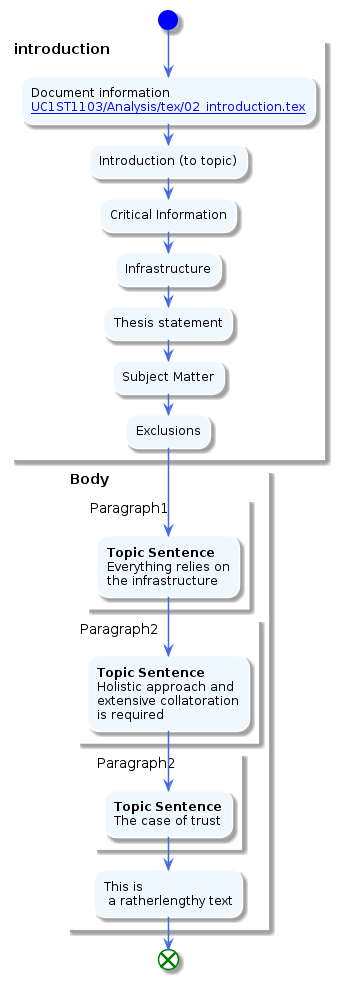
\includegraphics{tex/Studio_1_Activity_Diagram.png}





  \newpage
  \appendix
  \section{Appendix}

This is the appendix

  % bibliography
  \newpage
  % \clearpage
  % \input{tex/06_bibliography.tex}

  \section{Bibliography}
  \printbibliography

\end{document}